% This file was created by tikzplotlib v0.9.8.
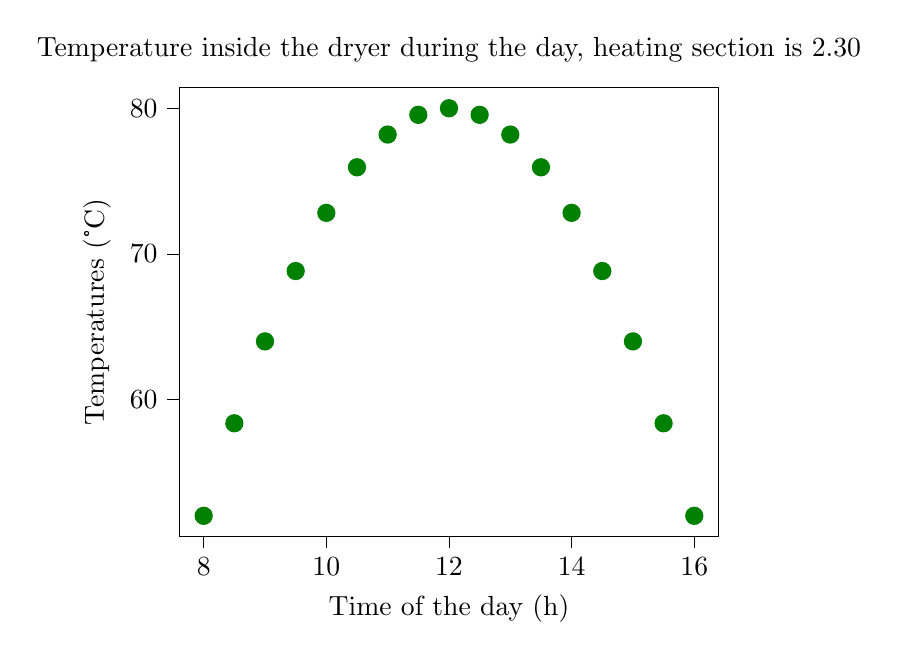
\begin{tikzpicture}

\begin{axis}[
tick align=outside,
tick pos=left,
title={Temperature inside the dryer during the day, heating section is 2.30},
x grid style={white!69.0196078431373!black},
xlabel={Time of the day (h)},
xmin=7.6, xmax=16.4,
xtick style={color=black},
y grid style={white!69.0196078431373!black},
ylabel={Temperatures (°C)},
ymin=50.5826105079109, ymax=81.4371129070949,
ytick style={color=black}
]
\addplot [semithick, green!50!black, mark=*, mark size=3, mark options={solid}, only marks]
table {%
8 51.985087889692
8.5 58.3536929549824
9 63.9905442886205
9.5 68.8315259893938
10 72.8348744515769
10.5 75.9724871396651
11 78.2255001415487
11.5 79.5818067345351
12 80.0346355253138
12.5 79.5818067345351
13 78.2255001415487
13.5 75.9724871396651
14 72.8348744515769
14.5 68.8315259893938
15 63.9905442886205
15.5 58.3536929549824
16 51.985087889692
};
\end{axis}

\end{tikzpicture}
